\vspace{0.3cm}
\begin{problema}
    (3 puntos) Se tiene una caja con 10 pelotas negras y 16 pelotas blancas. Se desean seleccionar 4 pelotas para una actividad pero de tal manera que la cantidad de pelotas negras y blancas no sean la misma ¿De cuántas maneras es posible realizar la selección?
\end{problema}


\vspace{0.3cm}




\begin{problema}
    (3 puntos) Dibuja una cuadrícula cuya cantidad de caminos de longitud mínima sea igual a la especificada en cada caso.

    
     \renewcommand{\theenumi}{\alph{enumi})}
    \begin{enumerate}
        \item $\binom{6}{2}$
        \item $\binom{5}{3}\binom{6}{2}$
        \item $\binom{6}{2}\binom{4}{1}+\binom{5}{1}$
    \end{enumerate}
    \renewcommand{\theenumi}{\arabic{enumi}}
\end{problema}

\vspace{0.3cm}



\begin{problema}
(3 puntos) Dada la siguiente cuadrícula, determina la cantidad de caminos que van del punto $A$ al punto $B$ si sólo se permiten movimientos hacia abajo y hacia la derecha.

\begin{center}
    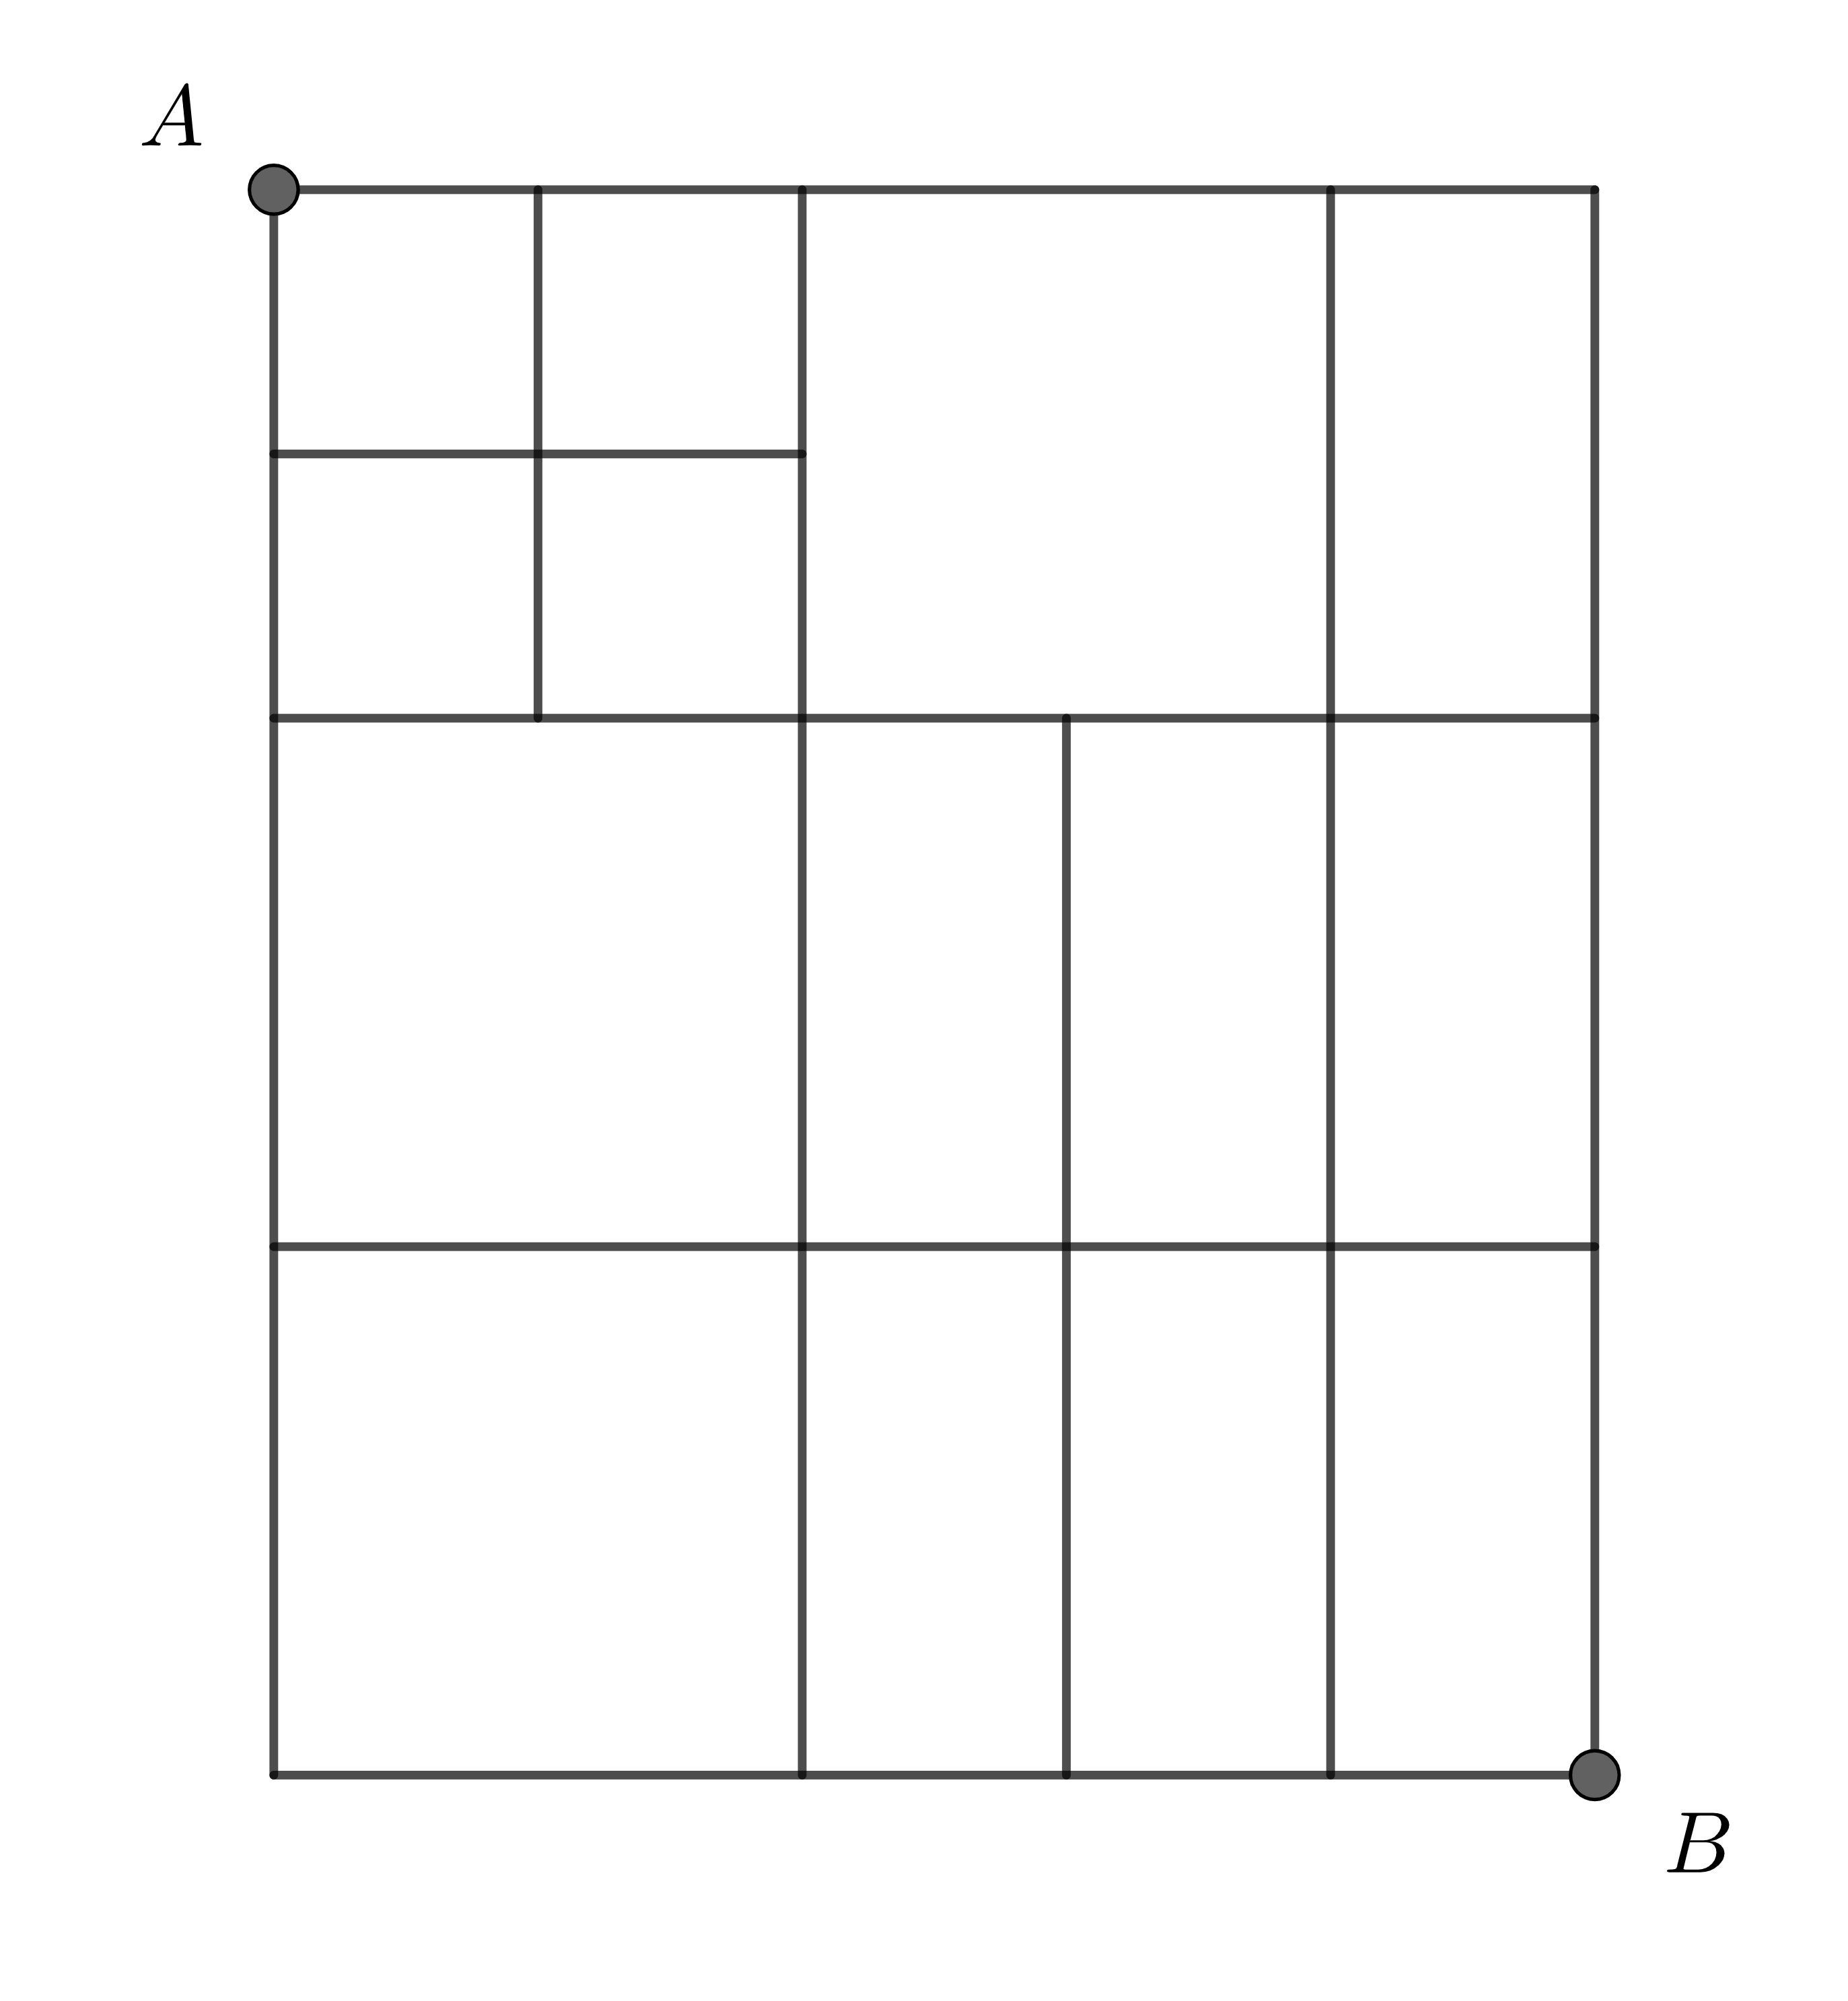
\includegraphics[scale=0.7]{Imagenes/IMG4/S1C4_Cuadricula.png}
\end{center}

\end{problema} 

\newpage


\begin{problema}
    (1 punto) Crea un meme usando la siguiente plantilla. \vspace{3cm}

        \begin{center}
            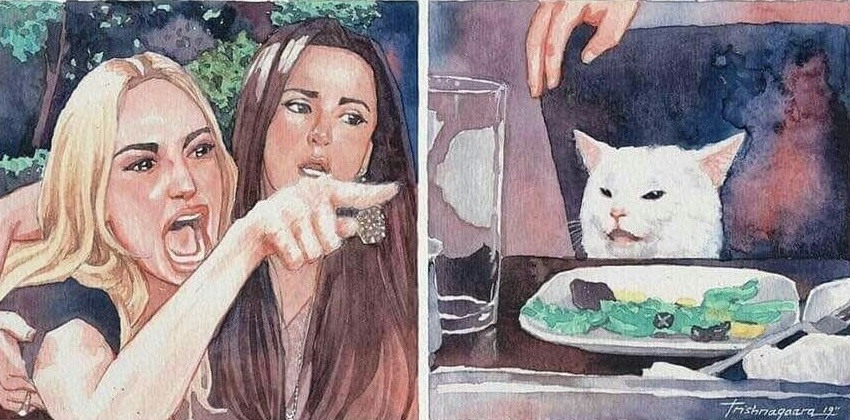
\includegraphics[scale=0.7]{Imagenes/IMG4/mujer-gritando-gato-en-la-mesa11567202426.jpg}
        \end{center}

    
\end{problema}\vspace{2cm}


\textbf{Crédito extra:}  La superficie de una caja se ha recubierto con una malla tal y como se puede observar en la imagen. Determina la cantidad de caminos de A a B sobre la malla si solamente se permite hacer movimientos hacia abajo a a la derecha.
\vspace{0.5cm}
\begin{center}
    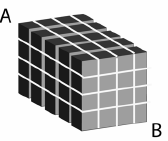
\includegraphics[scale=1]{Imagenes/IMG4/c9.PNG}
\end{center}
